\chapter{Introduction into bacterial interactions}
Interactions in natural microbial communities are a very common phenomenon, yet replicating such communities in a controlled environment is challenging, and therefore the impact of such interactions on single species or whole communities is often overlooked. Such interactions are often classified on the basis of their benefits for the respective interacting partners. This thesis describes two projects studying antagonistic interactions, namely antibiotic production and phage-bacteria interactions. 

\begin{figure}
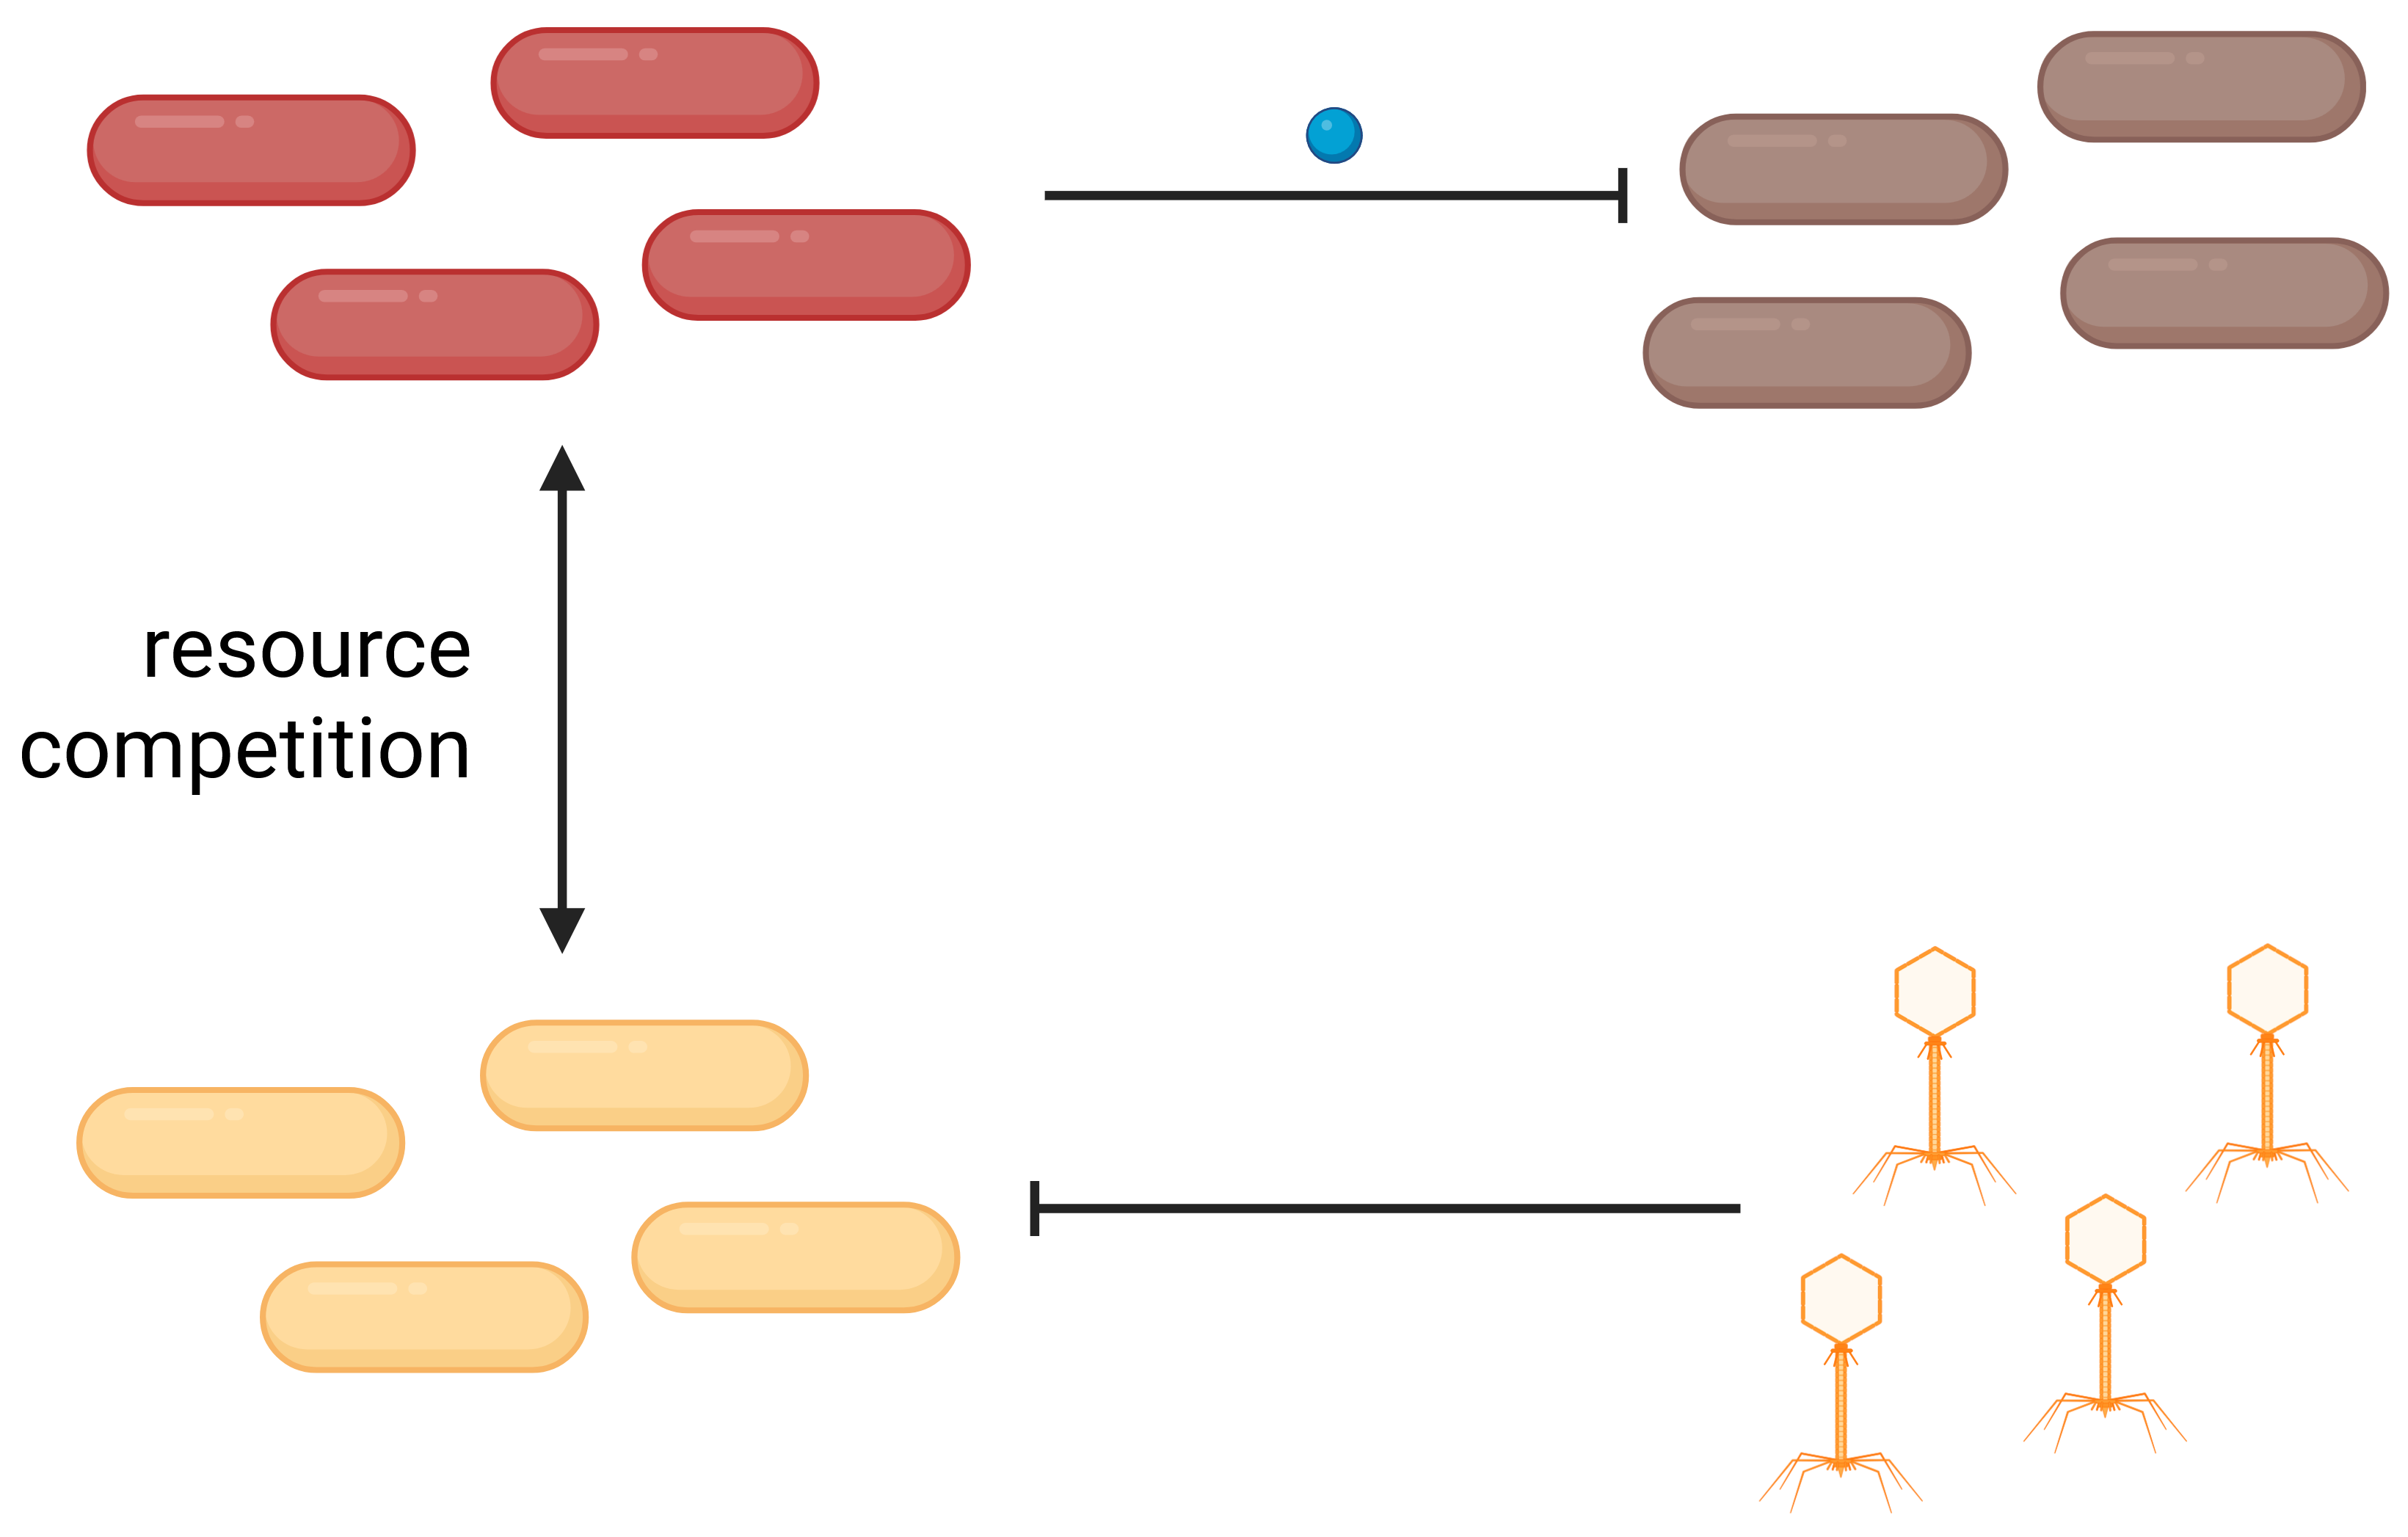
\includegraphics[width=\linewidth]{graphics/2025_09_28_intro_fig1.png}
\caption{\textbf{Antagonistic interactions studied in projects in this thesis} This sketch shows two common antagonistic interactions in microbial communities. The upper part of the sketch shows the production of a toxin (blue sphere) by a bacterial population which can then inhibit another target strain, sensitive to the produced toxin. At the same time there are other members in the community which compete for available resources such as nutrients. This interaction will be studied in the first, experimental project of this thesis. The lower part of the sketch shows the infection of a bacterial species by phages. Phage infections form an integral, important part of natural ecology. In addition to the phaage infection threat, the bacteria are in resource competition with phage-resistant bacteria. This bacteria-phage interaction will be studied in the second, theoretical project of this thesis.}
\label{fig:intro_shared_interactions}
\end{figure}